% Options for packages loaded elsewhere
\PassOptionsToPackage{unicode}{hyperref}
\PassOptionsToPackage{hyphens}{url}
\documentclass[
]{article}
\usepackage{xcolor}
\usepackage{amsmath,amssymb}
\setcounter{secnumdepth}{-\maxdimen} % remove section numbering
\usepackage{iftex}
\ifPDFTeX
  \usepackage[T1]{fontenc}
  \usepackage[utf8]{inputenc}
  \usepackage{textcomp} % provide euro and other symbols
\else % if luatex or xetex
  \usepackage{unicode-math} % this also loads fontspec
  \defaultfontfeatures{Scale=MatchLowercase}
  \defaultfontfeatures[\rmfamily]{Ligatures=TeX,Scale=1}
\fi
\usepackage{lmodern}
\ifPDFTeX\else
  % xetex/luatex font selection
\fi
% Use upquote if available, for straight quotes in verbatim environments
\IfFileExists{upquote.sty}{\usepackage{upquote}}{}
\IfFileExists{microtype.sty}{% use microtype if available
  \usepackage[]{microtype}
  \UseMicrotypeSet[protrusion]{basicmath} % disable protrusion for tt fonts
}{}
\makeatletter
\@ifundefined{KOMAClassName}{% if non-KOMA class
  \IfFileExists{parskip.sty}{%
    \usepackage{parskip}
  }{% else
    \setlength{\parindent}{0pt}
    \setlength{\parskip}{6pt plus 2pt minus 1pt}}
}{% if KOMA class
  \KOMAoptions{parskip=half}}
\makeatother
\usepackage{longtable,booktabs,array}
\usepackage{calc} % for calculating minipage widths
% Correct order of tables after \paragraph or \subparagraph
\usepackage{etoolbox}
\makeatletter
\patchcmd\longtable{\par}{\if@noskipsec\mbox{}\fi\par}{}{}
\makeatother
% Allow footnotes in longtable head/foot
\IfFileExists{footnotehyper.sty}{\usepackage{footnotehyper}}{\usepackage{footnote}}
\makesavenoteenv{longtable}
\usepackage{graphicx}
\makeatletter
\newsavebox\pandoc@box
\newcommand*\pandocbounded[1]{% scales image to fit in text height/width
  \sbox\pandoc@box{#1}%
  \Gscale@div\@tempa{\textheight}{\dimexpr\ht\pandoc@box+\dp\pandoc@box\relax}%
  \Gscale@div\@tempb{\linewidth}{\wd\pandoc@box}%
  \ifdim\@tempb\p@<\@tempa\p@\let\@tempa\@tempb\fi% select the smaller of both
  \ifdim\@tempa\p@<\p@\scalebox{\@tempa}{\usebox\pandoc@box}%
  \else\usebox{\pandoc@box}%
  \fi%
}
% Set default figure placement to htbp
\def\fps@figure{htbp}
\makeatother
\setlength{\emergencystretch}{3em} % prevent overfull lines
\providecommand{\tightlist}{%
  \setlength{\itemsep}{0pt}\setlength{\parskip}{0pt}}
\usepackage[margin=1in]{geometry}
\usepackage{booktabs}
\usepackage{longtable}
\usepackage{array}
\usepackage{microtype}
\usepackage{xcolor}
\setlength{\parskip}{0.5em}
\setlength{\parindent}{0pt}
\renewcommand{\arraystretch}{1.05}

% hyperref is loaded by pandoc's template AFTER this header. Use
% \AtBeginDocument to defer hypersetup until hyperref is present.
\AtBeginDocument{\hypersetup{colorlinks=true, linkcolor=black, urlcolor=blue, citecolor=blue}}

% Tighten footnote spacing
\setlength{\footnotesep}{0.4em}
\usepackage{bookmark}
\IfFileExists{xurl.sty}{\usepackage{xurl}}{} % add URL line breaks if available
\urlstyle{same}
\hypersetup{
  pdftitle={Digital Payments and Financial Inclusion in India: A State-Level Look at the Early and Mature UPI Eras},
  pdfauthor={Hari Dharshini Koundinya Swaminathen},
  hidelinks,
  pdfcreator={LaTeX via pandoc}}

\title{Digital Payments and Financial Inclusion in India: A State-Level
Look at the Early and Mature UPI Eras}
\usepackage{etoolbox}
\makeatletter
\providecommand{\subtitle}[1]{% add subtitle to \maketitle
  \apptocmd{\@title}{\par {\large #1 \par}}{}{}
}
\makeatother
\subtitle{A State-Level Look at the Early and Mature UPI Eras}
\author{Hari Dharshini Koundinya Swaminathen}
\date{}

\begin{document}
\maketitle

\section{1. Executive summary}\label{executive-summary}

Across Indian states in two distinct stretches of UPI's evolution,
financial-inclusion programmes that explicitly decouple account access
from income leave a measurable footprint on per-capita digital-payment
use. Programmes whose access scales with income, bank-office expansion,
telecom buildout, urban agglomeration, do not, because their cross-state
variation is absorbed by state income. This is the substantive read of
two parallel regressions, five years apart, with different dependent
variables, that give the same answer.

The two regressions cover the early-UPI era of FY 2019-20 and FY
2020-21, when UPI was one of five rails making up India's
digital-payment stack, and the mature-UPI era of April 2023 through
January 2026, when UPI alone settled the bulk of retail digital
payments. Both use the same four state-level controls (per-capita state
domestic product, urban share, PMJDY beneficiaries per adult,
bank-office density), the same estimator (pooled OLS with year fixed
effects and state-clustered standard errors), and the same log--log
specification.

\textbf{Three findings hold across both eras:}

\begin{itemize}
\item
  Per-capita state income is the dominant cross-state correlate of
  digital-payment use, with an elasticity close to one in both
  regressions. The two estimates are statistically indistinguishable
  from each other.
\item
  PMJDY beneficiary density adds explanatory power beyond income, with a
  positive elasticity statistically distinguishable from zero in both
  regressions (≈ +0.50 in the early era, ≈ +0.34 in the mature era).
  Conditional on income, states with broader PMJDY enrollment per adult
  use more digital payments per capita.
\item
  Bank-office density, urban share, and (in the mature era) internet
  penetration do not survive the income control in either regression.
  They correlate with digital-payment use unconditionally but not
  separably from the income gradient.
\end{itemize}

The cross-state distribution is also narrowing. The coefficient of
variation in monthly per-capita UPI declines at roughly 10 percent per
year over the 34-month panel; the standard deviation of log per-capita
UPI traces a parallel decline. Convergence is real, but a sixfold gap
between the highest-use and lowest-use states persists at the end of the
panel.

\textbf{Limits.} The findings are descriptive cross-state correlations
after controlling for income, not causal effects. The PMJDY result, the
firmest conditional finding, is associational. Section 5 sketches the
data and identification strategies that would let stronger claims
follow.

\section{2. Why this question matters}\label{why-this-question-matters}

In January 2026, India processed 21.7 billion UPI transactions worth
₹28.33 lakh crore. That was a 28 percent increase over the same month a
year earlier, and works out to roughly 700 million transactions every
day.\footnote{National Payments Corporation of India, UPI Product
  Statistics, https://www.npci.org.in/what-we-do/upi/product-statistics.
  The January 2026 figures are reported in NPCI's monthly press release
  and in the business press (e.g., DD News and Business Standard, 1
  February 2026).} UPI is now the largest retail payments system in the
world by volume. In a single month it settles more transactions than the
card networks of many large economies process in an entire year. The
Indian government and the National Payments Corporation of India (NPCI),
which operates the rail, regularly point to this scale as evidence that
digital payments have meaningfully advanced financial inclusion.

That January 2026 figure is the latest point in a longer story. The
story splits into two stretches worth analysing separately. The first is
the early-UPI era of FY 2019-20 and FY 2020-21. UPI was one of several
rails competing for digital-payment volume in that period. The
state-level data publishes only a five-rail composite (BHIM + IMPS +
RuPay POS + UPI + USSD). The second is the mature-UPI era from April
2023 through January 2026. By then UPI alone settled the bulk of retail
digital payments, and state-level pure-UPI data became consistently
available. Across the most recent twelve months (February 2025 through
January 2026), the 36 states and union territories of India together
processed about 142 billion state-attributable UPI transactions worth
₹197 lakh crore. That works out to roughly 8.3 transactions per person
per month, weighted by population.\footnote{Author's calculation from
  the panel constructed for this note. NPCI's all-India figure exceeds
  the state-summed total because a non-trivial share of transactions are
  reported under ``Unclassified'' and cannot be attributed to a specific
  state. The implications for the state-level analysis are discussed in
  section 3.} This note compares the two eras using a single set of
state-level controls. That way, what changed about who uses digital
payments, and what stayed the same, is visible in the coefficients.

\subsection{The national average hides the state-level
variation}\label{the-national-average-hides-the-state-level-variation}

The national figure of 8.3 monthly transactions per person hides a wide
range across states. Tripura sits at the bottom with 3.4. Telangana and
Goa sit at the top, both at 22.0. The gap is more than six-fold. The
most-used states do about five times the per-capita volume of the most
populous low-use states (figure 2, table 1). A national average that
hides variation this large cannot tell us whether UPI's scale has
reached people broadly. For policy purposes, the state is the right
unit. Payments infrastructure, regulations, and inclusion programs are
rolled out and evaluated at the state level. The populations they reach
differ in ways a national average smooths over.

\subsection{Two readings of the gap, both
true}\label{two-readings-of-the-gap-both-true}

The cross-state distribution can be read two ways. A useful policy
account of UPI needs to hold both readings at once.

The first reading is that states are converging. Between April 2023 and
January 2026, the cross-state coefficient of variation in monthly
per-capita UPI fell by roughly ten percent per year. The standard
deviation of log per-capita UPI fell at a similar rate (figure 4). In
plain terms: low-use states are growing their per-capita UPI faster than
high-use states are. The gap is closing.

The second reading is that the gap is still very large. The highest-use
states do five to eight times what the lowest-use states do. The gap is
narrowing, but it is far from closed.

\subsection{Why a financial-inclusion lens,
specifically}\label{why-a-financial-inclusion-lens-specifically}

UPI is routinely cited as a financial-inclusion success. But ``UPI
scaled'' and ``UPI scaled inclusively'' are different claims, and the
second is the more demanding one. The inclusion-relevant questions are
state-comparable. Do states with more PMJDY beneficiaries, accounts
opened under the government's flagship financial-inclusion scheme,
actually use digital payments more? Does the density of bank branches
and offices, the older form of financial-rail expansion, predict use in
the same way that account access does? Does the income gradient absorb
everything else once it is conditioned on? And do the answers look the
same in the early and mature UPI eras, or has the relationship shifted
as the rail matured? A two-period state-level analysis can answer these
questions; a national time series cannot.

\subsection{What this note does}\label{what-this-note-does}

Section 3 sets the empirical stage with the cross-state snapshot for the
most recent twelve months and the trend across the full 34 months of
mature-era data. Section 4 presents three findings about what predicts
state-level digital-payment use, each supported by two parallel
regressions, one for the early-UPI era (FY 2019-20 and FY 2020-21) using
the five-rail composite, one for the mature-UPI era (April 2023 through
January 2026) using pure UPI data. Both regressions use the same set of
state-level controls so the cross-era pattern is visible in the
coefficients. Section 5 takes up what the findings imply for
digital-payments and financial-inclusion policy. Methodology, full
regression tables, and a diagnostic on one variable (literacy) that we
set aside on measurement-validity grounds are in Appendix A; data
sources and construction notes are in Appendix B.

\section{3. The state-level landscape}\label{the-state-level-landscape}

This section sets the empirical stage in two parts. The first half is
the cross-state snapshot at the most recent twelve months for which we
have data, February 2025 through January 2026. The second half is the
trend across the full 34 months of mature-era data, asking whether the
cross-state distribution has been narrowing, widening, or holding
steady. The findings in Section 4 are read against this landscape.

\subsection{The state ranking}\label{the-state-ranking}

Figure 2 ranks the 36 states and union territories by their average
monthly per-capita UPI transactions over the most recent twelve months
(February 2025 -- January 2026), coloured by income quartile. Telangana
sits at the top with 22.0 monthly transactions per person, essentially
tied with Goa (22.0). Delhi (21.7) and Chandigarh (21.4) follow closely;
Maharashtra is fifth at 16.6. The bottom of the distribution is
dominated by the most populous low-income states and the small
north-eastern states: Tripura (3.4), Bihar (3.5), Manipur (4.4),
Jharkhand (4.4), and Meghalaya (4.4). The India population-weighted
average, the figure a national reader would normally cite, is 8.3
transactions per person per month, marked on the figure by the dashed
vertical line.

The income-tier colouring makes the cross-state pattern visible at a
glance. The upper half of the ranking is overwhelmingly the dark blue of
the upper income quartile, and the lower half is overwhelmingly the dark
red of the lowest quartile. Two pairs of states sit visibly off the
diagonal. Gujarat and Himachal Pradesh, both upper-mid-income states,
show up in the lower half of the per-capita UPI ranking, well below
where their income tier alone would predict. Andhra Pradesh and
Arunachal Pradesh, both in the lower-mid-income tier, show up in the
upper half, well above what their income tier alone would predict. These
four are visible exceptions to the broad income--UPI association, but
they remain exceptions: across the full set, income tier is the dominant
predictor of where a state sits, which is what the regression in Section
4 quantifies formally.

\subsection{The summary statistics}\label{the-summary-statistics}

Table 1 summarises the seven variables that enter the cross-state
analysis: per-capita UPI use (the dependent variable), the five
regression controls (per-capita NSDP, internet density, urban share,
PMJDY beneficiaries per adult, bank-office density), and the
appendix-only literacy variable. For each variable we report the
cross-state mean, standard deviation, minimum and maximum, and the
population-weighted India-wide value.

Three patterns in the table are worth pulling out, because they
illustrate how cross-state averages can diverge from population-weighted
national figures and what that divergence reveals.

Per-capita UPI use has a state mean of 9.6 monthly transactions per
person but a population-weighted India figure of 8.3. The gap is small
but goes in a specific direction: the highest-use states are mostly not
the most populous ones. Telangana, Chandigarh, Delhi, and Goa are
smaller in population than their UPI rank would suggest, while Uttar
Pradesh and Bihar, large and populous, sit toward the bottom. The state
mean overstates the typical Indian's per-capita UPI use; the
population-weighted figure is the more honest reading of the national
level.

PMJDY beneficiaries per adult shows the opposite pattern. The state mean
is 0.41 accounts per adult, but the population-weighted figure is 0.53.
The difference is large and reflects exactly what PMJDY's targeting was
designed to do: enrollment is highest in populous low-income states
(Bihar at 0.75, Jharkhand at 0.69, Madhya Pradesh at 0.68, Rajasthan at
0.61, Uttar Pradesh at 0.59). When we weight by population, those states
pull the national figure up well above the cross-state mean. The same
scheme that looks modest as a state-level mean (41 percent of adults) is
a much larger national effort when measured in adult-weighted terms (53
percent of adults).

Bank-office density per 100,000 population shows the same direction as
per-capita UPI use: state mean of 17.9 per 100k, population-weighted
India figure of 12.4. Small states and union territories have many more
bank offices per person than large states do (Goa at 46, Lakshadweep at
40, Chandigarh at 39, Ladakh at 35, Sikkim at 27, Himachal Pradesh at
25; the largest states sit between 8 and 12). The state-mean figure
should not be mistaken for the average Indian's access to a bank office,
it overstates that average by close to 50 percent.

The remaining variables move less between state mean and
population-weighted figure because they are more uniformly distributed:
urban share (46.5 percent state mean, 36.1 percent population-weighted;
the population-weighted figure pulls down because rural states are
populous), literacy (85.6 vs 80.8 percent), internet density (80.4 vs
68.6 subscribers per 100), and per-capita NSDP (₹146,000 vs ₹116,000).

\subsection{And the gap is closing}\label{and-the-gap-is-closing}

The snapshot is at the most recent twelve months, but the cross-state
distribution has been moving over the full 34-month window for which we
have monthly state-level UPI data, April 2023 through January 2026.
Figure 4 plots two complementary dispersion measures over that window,
each indexed to its own value at panel start. Both narrow steadily.

The cross-state coefficient of variation in monthly per-capita UPI
declines at roughly 10 percent per year, ending the panel about 27
percent below its April 2023 starting value. The standard deviation of
log per-capita UPI declines at roughly 8 to 9 percent per year, ending
about 24 percent below its starting value. The two measures track each
other closely, the convergence finding does not depend on which one you
choose. In plain terms: low-use states are growing their per-capita UPI
faster than high-use states are. The gap is closing.

A useful way to think about the magnitude. At the panel-start level of
dispersion, the highest-use state did about ten times the per-capita
volume of the lowest-use state. By January 2026 that ratio had fallen
closer to seven. The gap is still large, convergence is not parity, but
the trend over thirty-four months is steady downward narrowing. Two
robustness checks on the convergence pattern are in Appendix B: a test
of whether the growing ``Unclassified'' share of national UPI volume is
concentrated in particular states (it is not, statistically), and a note
on Maharashtra's six-percentage-point share loss over the panel period
(which contributes to the narrowing but does not drive it).

\subsection{Reading these levels into the
findings}\label{reading-these-levels-into-the-findings}

The level of cross-state variation in per-capita UPI use is large. A
more-than-six-fold gap between the lowest- and highest-use states is not
a rounding error around the national average. The convergence trend is
real, but it is operating against an initial dispersion of meaningful
magnitude. Section 4 takes up which state-level variables predict where
states sit in this distribution.

\subsection{Figure 2 --- State ranking by per-capita UPI use, most
recent twelve months (Feb 2025 -- Jan
2026)}\label{figure-2-state-ranking-by-per-capita-upi-use-most-recent-twelve-months-feb-2025-jan-2026}

\pandocbounded{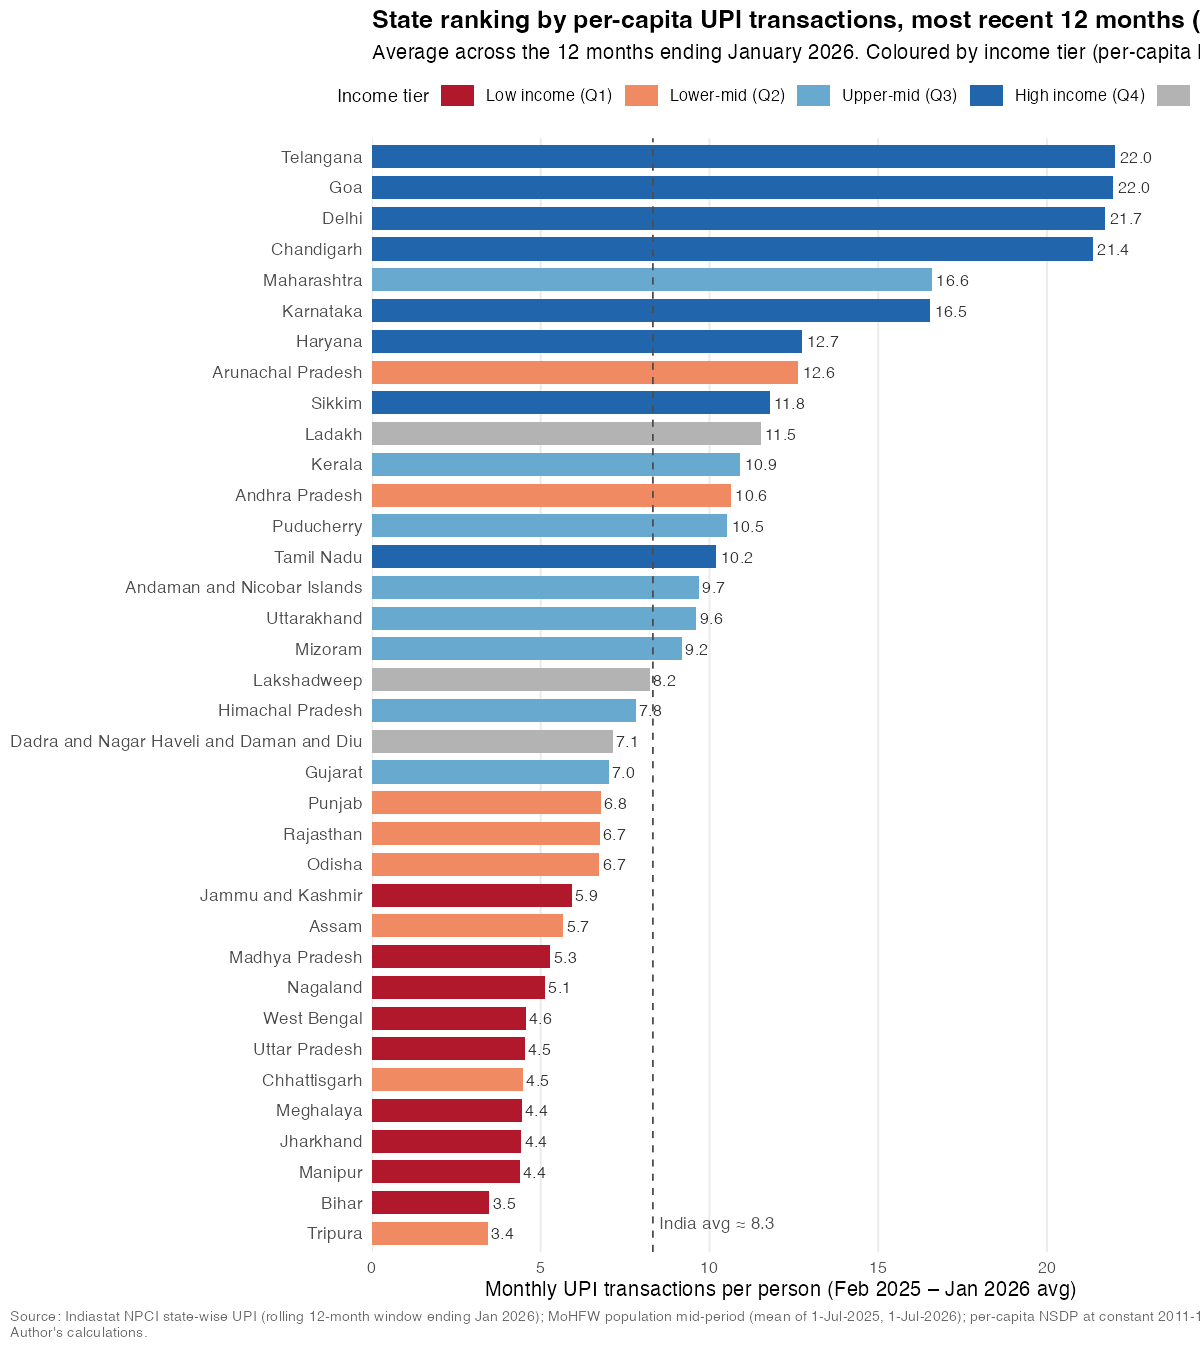
\includegraphics[keepaspectratio]{figures/fig2_state_ranking_w3.png}}

\subsection{Table 1 --- Descriptive statistics, most recent twelve
months (Feb 2025 -- Jan
2026)}\label{table-1-descriptive-statistics-most-recent-twelve-months-feb-2025-jan-2026}

\begin{longtable}[]{@{}
  >{\raggedright\arraybackslash}p{(\linewidth - 14\tabcolsep) * \real{0.4762}}
  >{\raggedright\arraybackslash}p{(\linewidth - 14\tabcolsep) * \real{0.1349}}
  >{\raggedleft\arraybackslash}p{(\linewidth - 14\tabcolsep) * \real{0.0238}}
  >{\raggedright\arraybackslash}p{(\linewidth - 14\tabcolsep) * \real{0.0635}}
  >{\raggedright\arraybackslash}p{(\linewidth - 14\tabcolsep) * \real{0.0556}}
  >{\raggedright\arraybackslash}p{(\linewidth - 14\tabcolsep) * \real{0.0556}}
  >{\raggedright\arraybackslash}p{(\linewidth - 14\tabcolsep) * \real{0.0635}}
  >{\raggedright\arraybackslash}p{(\linewidth - 14\tabcolsep) * \real{0.1270}}@{}}
\toprule\noalign{}
\begin{minipage}[b]{\linewidth}\raggedright
Variable
\end{minipage} & \begin{minipage}[b]{\linewidth}\raggedright
Unit
\end{minipage} & \begin{minipage}[b]{\linewidth}\raggedleft
N
\end{minipage} & \begin{minipage}[b]{\linewidth}\raggedright
Mean
\end{minipage} & \begin{minipage}[b]{\linewidth}\raggedright
SD
\end{minipage} & \begin{minipage}[b]{\linewidth}\raggedright
Min
\end{minipage} & \begin{minipage}[b]{\linewidth}\raggedright
Max
\end{minipage} & \begin{minipage}[b]{\linewidth}\raggedright
India (pop-wt.)
\end{minipage} \\
\midrule\noalign{}
\endhead
\bottomrule\noalign{}
\endlastfoot
Per-capita UPI transactions (Feb 2025 -- Jan 2026 avg) & per
person/month & 36 & 9.6 & 5.5 & 3.4 & 22.0 & 8.3 \\
Per-capita NSDP (latest available, constant 2011-12 prices) & INR & 33 &
146,389 & 76,268 & 36,342 & 357,611 & 116,350 \\
Internet subscribers (31-Mar-2025, latest TRAI release) & per 100
persons & 36 & 80.4 & 27.9 & 41.6 & 161.8 & 68.6 \\
Urban population share (interpolated to 2025) & \% & 35 & 46.5 & 25.1 &
10.4 & 100.0 & 36.1 \\
PMJDY beneficiaries per adult (snapshot 13-Dec-2025) & accounts / adult
& 36 & 0.41 & 0.20 & 0.09 & 0.91 & 0.53 \\
Bank offices per 100,000 population (31-Dec-2025) & per 100k pop & 36 &
17.9 & 9.6 & 6.5 & 46.2 & 12.4 \\
Literacy rate, persons 7+ (FY 2023-24, appendix only) & \% & 36 & 85.6 &
7.1 & 72.6 & 98.2 & 80.8 \\
\end{longtable}

\subsection{Figure 4 --- Cross-state dispersion in per-capita UPI, Apr
2023 -- Jan
2026}\label{figure-4-cross-state-dispersion-in-per-capita-upi-apr-2023-jan-2026}

\pandocbounded{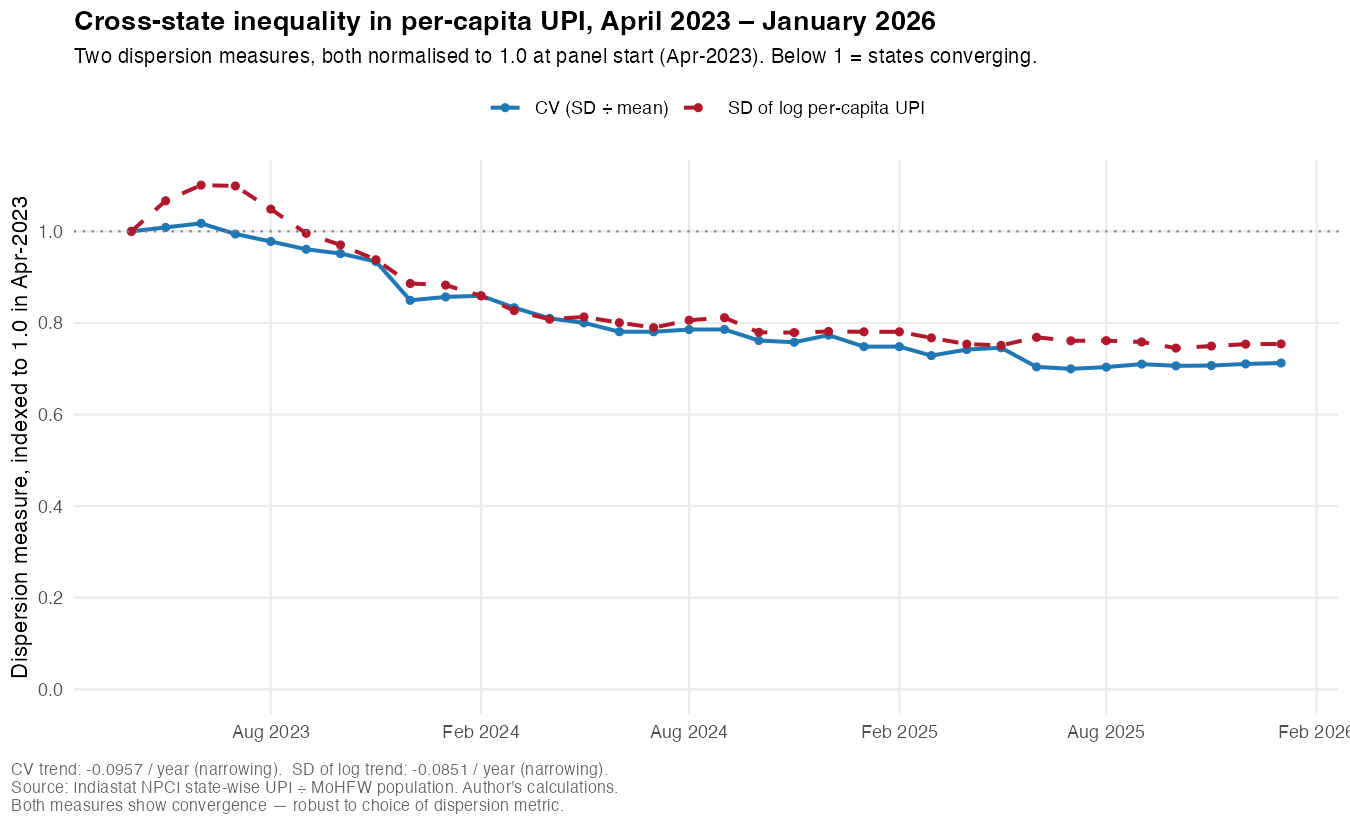
\includegraphics[keepaspectratio]{figures/fig4_convergence.png}}

\section{4. What predicts state-level digital-payment
use}\label{what-predicts-state-level-digital-payment-use}

This section presents three findings about what predicts state-level
digital-payment use across Indian states. Each finding is supported by
two parallel regressions: the early-UPI era of FY 2019-20 and FY
2020-21, when UPI was one of five rails making up India's
digital-payment stack, and the mature-UPI era of April 2023 through
January 2026, when UPI alone settled the bulk of retail digital
payments. Both regressions use the same four state-level controls
(per-capita state domestic product, urban population share, PMJDY
beneficiaries per adult, and bank-office density), the same estimator
(pooled OLS with year fixed effects and standard errors clustered at the
state level), and the same log--log specification. The mature-era
regression adds a fifth control, internet density, that becomes
available only in that period.

Full methodology, regression specifications, and detailed result tables
are in Appendix A. Table 2 below summarises the headline coefficients on
the four shared controls in both eras; the rest of this section walks
through what the table makes visible.

\subsection{Table 2, Cross-era coefficients on the four shared
controls}\label{table-2-cross-era-coefficients-on-the-four-shared-controls}

\begin{longtable}[]{@{}
  >{\raggedright\arraybackslash}p{(\linewidth - 4\tabcolsep) * \real{0.2727}}
  >{\raggedleft\arraybackslash}p{(\linewidth - 4\tabcolsep) * \real{0.3636}}
  >{\raggedleft\arraybackslash}p{(\linewidth - 4\tabcolsep) * \real{0.3636}}@{}}
\toprule\noalign{}
\begin{minipage}[b]{\linewidth}\raggedright
Control
\end{minipage} & \begin{minipage}[b]{\linewidth}\raggedleft
Early-UPI era (FY 2019-20 + 2020-21)
\end{minipage} & \begin{minipage}[b]{\linewidth}\raggedleft
Mature-UPI era (Apr 2023 -- Jan 2026)
\end{minipage} \\
\midrule\noalign{}
\endhead
\bottomrule\noalign{}
\endlastfoot
log(per-capita NSDP) & \textbf{+1.17} ** & \textbf{+1.05} *** \\
log(urban share) & +0.25 & +0.06 \\
log(PMJDY beneficiaries / adult) & \textbf{+0.50} * & \textbf{+0.34}
** \\
log(bank offices / 100k pop) & −0.17 & −0.19 \\
Sample size (state-period observations) & 66 & 99 \\
\end{longtable}

Bold figures are statistically distinguishable from zero. Significance:
* p\textless0.10, ** p\textless0.05, *** p\textless0.01. Coefficients
are elasticities, a 1 percent change in the control is associated with a
β-percent change in per-capita digital-payment use, holding the other
controls constant.

\subsection{Finding 1: Income is the dominant correlate, in both
eras}\label{finding-1-income-is-the-dominant-correlate-in-both-eras}

The cleanest empirical pattern in the two regressions is the income
elasticity. In the early-UPI era it is +1.17, statistically significant
at the 5 percent level; in the mature-UPI era it is +1.05, significant
at the 1 percent level. Both are close to a unit elasticity. A 10
percent increase in a state's per-capita state domestic product is
associated with about a 10 percent increase in its per-capita
digital-payment use, and that relationship was already in place in
2019-21 and persisted essentially unchanged through 2024-25.

The two estimates are close enough that they are not statistically
distinguishable from each other. This is meaningful in itself. The
dependent variable in the early era was a five-rail composite (BHIM,
IMPS, RuPay-on-POS, UPI, USSD); in the mature era it is pure UPI. The
sample sizes differ; the panel structures differ; the controls differ in
one variable. Yet the income-elasticity is the same. Whatever else
changed about UPI between 2019 and 2026, the sheer scale of
transactions, UPI's displacement of the four other rails, the doubling
of bank-office counts, the addition of hundreds of millions of PMJDY
beneficiaries, the income gradient of digital-payment use has held its
shape.

Two readings follow. First, income is by far the most reliable predictor
of where a state will sit in the cross-state distribution of
digital-payment use, and any policy aimed at expanding digital payments
at the state level is operating against a strong income gradient.
Second, the durability of the relationship across two distinct
measurement regimes makes it unlikely that the income gradient is an
artefact of how the dependent variable is constructed in either era, it
is a feature of the underlying state-level distribution. The pattern is
associational, not causal; what it does establish is that any other
state-level variable claimed to matter for digital-payment use needs to
survive controlling for income. Findings 2 and 3 are both about which
variables clear that bar.

\subsection{Finding 2: Financial-inclusion programs (PMJDY) add
explanatory power beyond income, in both
eras}\label{finding-2-financial-inclusion-programs-pmjdy-add-explanatory-power-beyond-income-in-both-eras}

This is the policy-relevant finding of the analysis. The coefficient on
log(PMJDY beneficiaries per adult) is positive and statistically
distinguishable from zero in both regressions: +0.50 in the early-UPI
era (significant at the 10 percent level) and +0.34 in the mature-UPI
era (significant at the 5 percent level). A 10 percent relative increase
in PMJDY enrollment per adult is associated with a 3 to 5 percent
increase in per-capita digital-payment use, holding income, urban share,
bank-office density, and (in the mature era) internet density constant.
The two estimates are statistically indistinguishable from each other.

The finding has more bite than the magnitudes alone suggest, because the
univariate correlation between PMJDY enrollment and per-capita
digital-payment use is negative across Indian states (Pearson r in
log--log of about −0.42; see Figure 5). PMJDY-heavy states are poorer
states, and poorer states use digital payments less. So unconditionally,
more PMJDY enrollment looks associated with less digital-payment use.
The negative univariate correlation is income masquerading as PMJDY.

Once we control for income, the sign flips. Among states at similar
income levels, those with higher PMJDY enrollment per adult use more
digital payments. The flip is not a regression artefact, it is what the
data say once the income gradient is held constant. And the flip occurs
in both eras: when PMJDY had been running for five to six years and was
still in its build-out phase (early-UPI era), and when it had reached
close to a decade of cumulative enrollment (mature-UPI era).

\pandocbounded{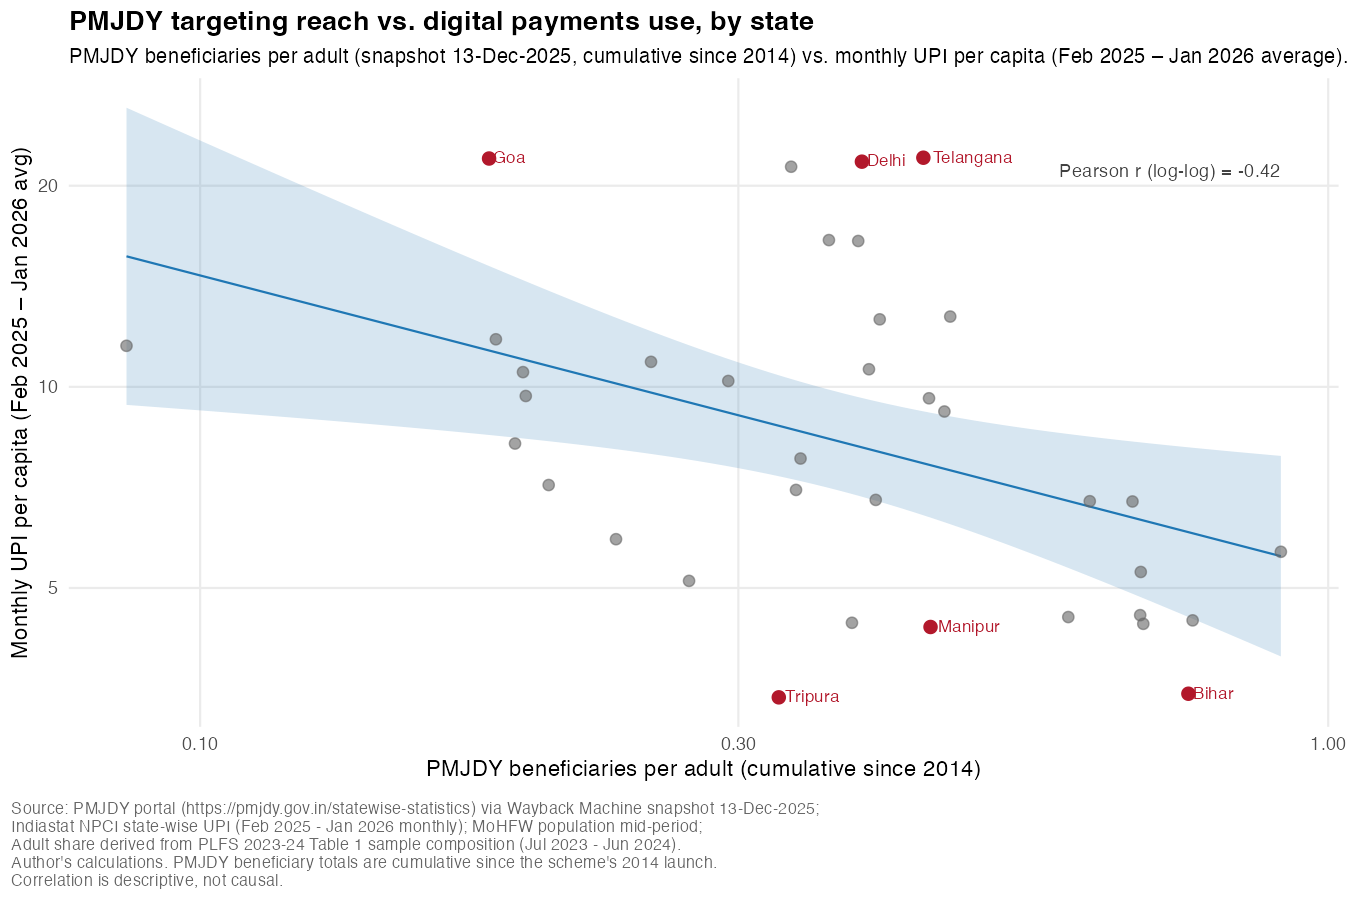
\includegraphics[keepaspectratio]{figures/fig5_pmjdy_vs_upi.png}}

The mechanism is account access. PMJDY's design opens a basic savings
account for unbanked households, and an account is the necessary
condition for using a digital-payment rail at all. The variable measures
the cumulative reach of that scheme, normalised by adult population. The
regression detects that this measure of account access predicts
digital-payment use beyond what income alone does, in both eras. The
reading is not that PMJDY caused UPI adoption, the data here cannot
establish that, but that programmatic financial inclusion has a durable
association with digital-payments use that survives the income control.

The policy implication, developed in Section 5, is straightforward:
financial-inclusion programs that decouple account access from income,
as PMJDY does, by deliberately targeting the unbanked, leave a
statistical footprint in cross-state digital-payment use. The same is
not true of every variable that captures financial inclusion, as Finding
3 shows.

\subsection{Finding 3: Financial-inclusion infrastructure (bank offices)
does not add beyond income, in either
era}\label{finding-3-financial-inclusion-infrastructure-bank-offices-does-not-add-beyond-income-in-either-era}

The contrast with PMJDY is sharp. The coefficient on log(bank offices
per 100,000 population) is small and statistically indistinguishable
from zero in both regressions: −0.17 in the early era, −0.19 in the
mature era. Bank-office density does not survive joint inclusion with
income. The same is true of urban share (+0.25 and +0.06, neither
significant) and, in the mature era where it is available, internet
density (+0.34, also not significant).

This is not because bank-office density is irrelevant to digital-payment
use. The univariate correlation between bank-office density and
per-capita UPI use is positive and substantial (Pearson r in log--log of
about +0.67; Figure 6). States with more banking infrastructure per
person do use more digital payments per person, in the unconditional
cross-section.

\pandocbounded{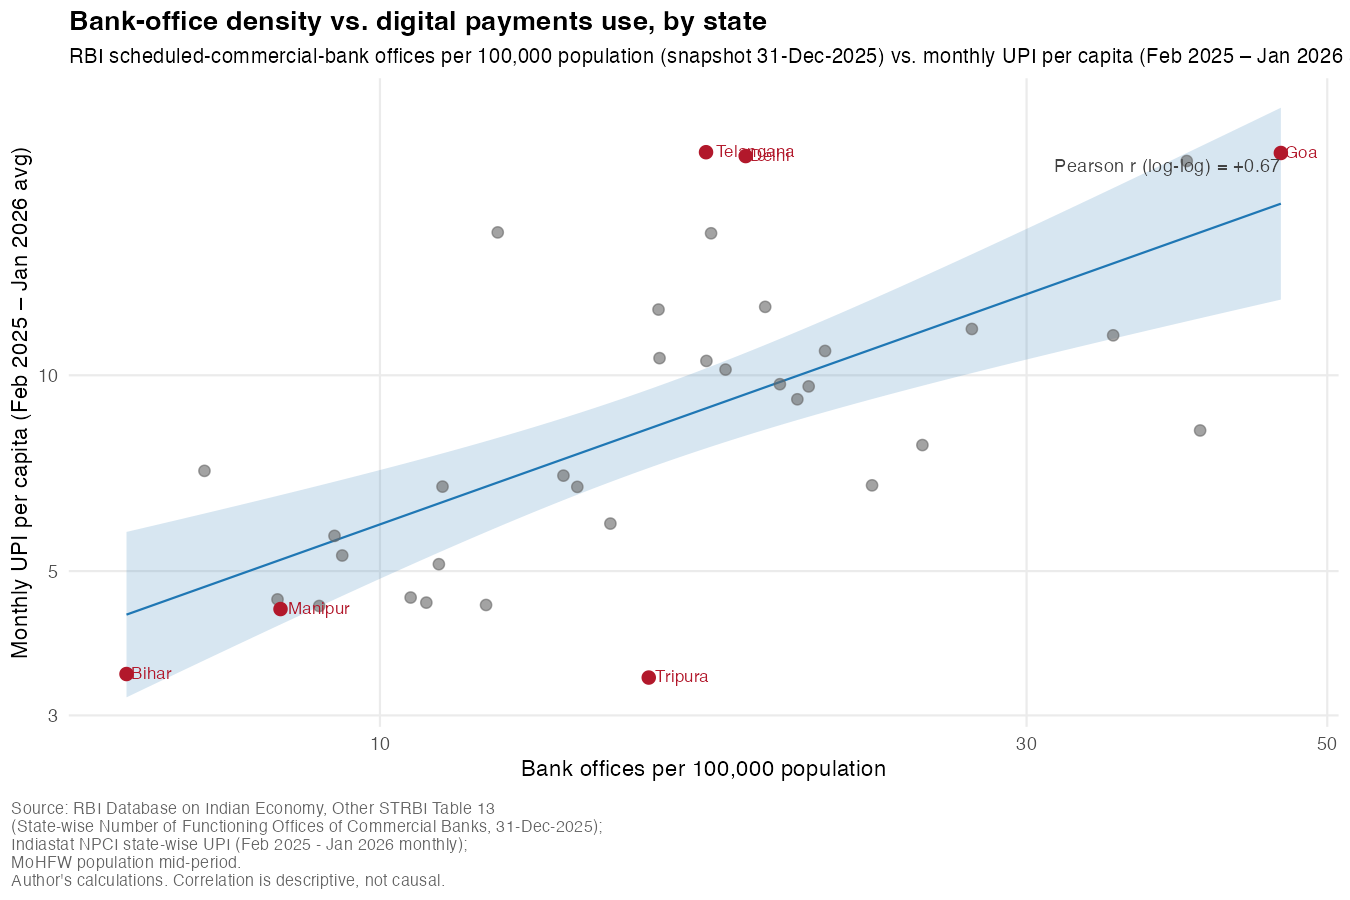
\includegraphics[keepaspectratio]{figures/fig6_bank_offices_vs_upi.png}}

The reason the conditional coefficient is null is collinearity with
state income. In the cross-section of Indian states, bank-office density
correlates with per-capita NSDP at roughly +0.85; urban share correlates
with NSDP at roughly +0.7; internet density correlates with NSDP at
+0.86. All three variables capture economically real and theoretically
distinct channels, physical banking infrastructure, urban agglomeration,
and telecom buildout, but they all move tightly with state income. Once
income is in the regression, the marginal contribution of any of these
variables beyond what NSDP already absorbs is statistically
indistinguishable from zero.

PMJDY survives this test for one structural reason. PMJDY enrollment per
adult correlates with per-capita NSDP at roughly −0.62, strongly
negatively. The scheme deliberately targets the unbanked, who are
concentrated in poorer states, so its beneficiary density runs in the
opposite direction from income. That negative correlation is precisely
what gives PMJDY identification beyond income: conditioning on income
does not collapse PMJDY's variation, because income and PMJDY move in
opposite directions across states.

The substantive distinction this draws is between two kinds of financial
inclusion. Financial-inclusion infrastructure, bank offices, telecom
buildout, urban agglomeration, is allocated by markets and grows with
state income. In our data, it shows up through the income gradient, not
beyond it. Financial-inclusion programs designed to reach the population
outside that gradient, PMJDY in our case, show up beyond income in a way
the regression can identify separately. This is the policy-relevant
distinction the next section takes up.

A note on what we set aside: a sixth state-level variable, literacy, was
tried in both eras and produced an interpretable pattern that we read as
a measurement-validity problem with the literacy variable as
conventionally defined rather than a substantive finding about literacy
and digital payments. The full diagnostic is in Appendix A.

\section{5. Policy implications}\label{policy-implications}

The findings in Section 4 carry three specific implications for
digital-payments and financial-inclusion policy. We take each in turn.

\subsection{1. Design financial-inclusion programmes to decouple access
from
income}\label{design-financial-inclusion-programmes-to-decouple-access-from-income}

The actionable read of the PMJDY result is that the kind of inclusion
design matters, not just the inclusion variable itself. Programmes that
deliberately decouple access from income, as PMJDY does, by targeting
the unbanked, leave a measurable footprint on cross-state
digital-payment use beyond what general economic development would
already produce. Programmes whose access scales with the market,
bank-office expansion, telecom buildout, urban agglomeration, do not,
because their cross-state variation is absorbed by the income gradient.
The mechanism is developed in Section 4, Finding 3.

The general claim that follows is not a finding about one scheme. It is
empirical evidence that the design of an inclusion programme, whether it
allocates by market or by deliberate counter-targeting, predicts whether
the programme will leave a measurable cross-state footprint on
digital-payment use. Programmes whose allocation rule moves with state
income will, in cross-state monitoring, look like income through a
different lens. Programmes that decouple from income may show up
separately.

The methodology generalises and the variable does not. Future work
should run the same cross-era, same-controls regressions on other
state-level inclusion programmes whose enrollment data exist: Direct
Benefit Transfer (DBT) volumes, Mudra credit coverage, Aadhaar-enabled
Payments System (AePS) uptake, and the targeted merchant-onboarding
programmes that BHIM and the National Payments Corporation of India have
run since 2017. Each of these has a state-level enrollment count that
could be measured against per-capita digital-payment use conditional on
income. The methodology in Appendix A is designed to be transportable to
any of them.

\subsection{2. State-level dispersion belongs in inclusion
monitoring}\label{state-level-dispersion-belongs-in-inclusion-monitoring}

The monthly all-India UPI volume that NPCI publishes, and that the press
and the government routinely cite, is the wrong figure for inclusion
monitoring. It averages over precisely the cross-state variation that is
the inclusion-relevant signal. A 21.7-billion-transaction national
headline (January 2026) coexists with an eight-fold gap between the
highest- and lowest-use Indian states. The headline tells you about
UPI's overall scale; it tells you essentially nothing about whether that
scale has reached the populations who were the target of inclusion
policy in the first place.

The cross-state coefficient of variation and the standard deviation of
log per-capita UPI are policy-relevant metrics. Both are easy to compute
monthly from the data NPCI already publishes, and both convey
information the national headline does not (Section 3, Figure 4). NPCI
and the Reserve Bank of India should publish these (or equivalent)
dispersion measures alongside the national volume in the monthly UPI
release. The inclusion-policy ecosystem cannot monitor distributional
progress on a metric that has not been made standard.

A linked data-quality concern: the share of monthly UPI volume reported
under ``Unclassified'', transactions that cannot be attributed to a
specific state, has grown from approximately 12 percent in April 2023 to
nearly 40 percent by January 2026. If two-fifths of national UPI volume
sits outside the state-level data, the state-level inclusion picture is
partially blind. Whatever the cause, Mumbai-routed payment
infrastructure, multi-state merchant attribution, or something else,
NPCI's reporting choices on the Unclassified bucket are an
inclusion-policy concern, not just a data engineering one.

\subsection{3. What this paper does not license, and what would
strengthen the
claim}\label{what-this-paper-does-not-license-and-what-would-strengthen-the-claim}

The findings here are cross-state and descriptive. They cannot establish
causation. Specifically: the bank-office null is a statement about
cross-state identification, not evidence that an additional bank office
in any particular place would not raise digital-payment use; the same
applies to the internet null. The PMJDY result, the firmest conditional
finding, is associational, we cannot rule out that PMJDY enrollment and
per-capita digital-payment use are jointly driven by state-level
political, cultural, or historical factors not in the regression.

Three extensions would substantially strengthen what we can claim.
District-level digital-payment data, not currently published at the
granularity we have for state level, would allow within-state analysis
that holds those unobservable factors constant. Causal designs that
exploit the state-by-state phasing of PMJDY's rollout between 2014 and
2020 could turn the associational finding into an identified treatment
effect. A state-level measure of digital literacy, smartphone
navigation, app fluency, comfort with numeric prompts, distinct from the
basic primary-language literacy variable our data contain, would resolve
the puzzle documented in Appendix A and possibly identify a separate
channel the current analysis cannot.

Until those data exist, the paper provides robust descriptive evidence
on cross-state correlates of digital-payment use across two distinct UPI
eras. The policy reads in this section follow from those patterns; they
do not exceed them.

\section{6. Conclusion}\label{conclusion}

The question this paper opened with was specific: across Indian states,
in two distinct stretches of UPI's evolution, what predicts state-level
digital-payment use, and what does the cross-era pattern imply for
inclusion policy?

The answer is built around three findings that hold in both eras. Income
is the dominant cross-state correlate of digital-payment use, with a
roughly unit elasticity in both regressions. PMJDY beneficiary density
adds explanatory power beyond income, with a positive elasticity that is
statistically distinguishable from zero in both eras and quantitatively
similar across them. Bank-office density, urban share, and (in the
mature era) internet penetration are absorbed by income, they correlate
with digital-payment use unconditionally, but not separably from the
income gradient. The cross-era stability itself is the meta-finding: the
same pattern shows up with a five-rail composite in 2019-21 and with
pure UPI in 2023-26, across different sample sizes and different time
structures.

That stability points to a specific reading of the inclusion question we
started with. Has UPI's scale translated into broad-based financial
inclusion? Partially yes, and the partial-yes is conditional on
programmes that deliberately decouple account access from income. Where
such programmes operate at scale, PMJDY is the case our data document,
they leave a measurable footprint on cross-state digital-payment use
that survives the income control. Where they do not, UPI's growth is
well-described as economic development, of which digital-payment
activity is one expression among many. The same income gradient that
explains state-level differences in education access, electricity
coverage, and consumption levels also explains state-level differences
in digital-payment use.

What we have established is a robust cross-state pattern. What we have
not established is causation; the data and designs that would let
stronger claims follow are sketched in Section 5. The cross-state record
from 2019 through 2026 is consistent with a policy hypothesis worth
testing. It does not yet test it.

\section{Appendix A. Methodology and detailed
results}\label{appendix-a.-methodology-and-detailed-results}

This appendix documents the estimator, sample, and full regression
results that the body of the memo summarises. Data sources and
construction are in Appendix B.

\subsection{A.1 Estimator and
specification}\label{a.1-estimator-and-specification}

The two regressions are pooled ordinary least squares with year fixed
effects (early-UPI era) or year-window fixed effects (mature-UPI era)
and standard errors clustered at the state level. The dependent variable
and all continuous controls are log-transformed; coefficients are
therefore elasticities. The fixed effects absorb the period-specific
national level so the regression identifies cross-state variation rather
than common time trends.

The early-UPI regression has four state-level controls: log(per-capita
NSDP), log(urban share), log(PMJDY beneficiaries per adult), and
log(bank offices per 100,000 population). The mature-UPI regression adds
a fifth, log(internet density per 100 population), that becomes
available only in that period. We do not run a within-state
specification: with most controls largely time-invariant in the
available data, state fixed effects would absorb the variation we are
trying to identify. The research design is cross-state across multiple
periods, with year/window FE absorbing common time trends.

The dependent variables are definitionally different across the two
regressions and are not chained. The early-era DV is per-capita
transactions on a five-rail composite (BHIM + IMPS + RuPay POS + UPI +
USSD); the mature-era DV is per-capita pure UPI. Each regression is
interpreted within its era; the cross-era comparison in A.5 reads
coefficients on the four shared controls, not the dependent variables
themselves.

A note on the timing of variables within a window. The dependent
variable in the mature-era regression is a 12-month average of monthly
per-capita UPI within each window. The state-level controls are not
12-month averages, they are point-in-time snapshots (PMJDY
beneficiaries, bank-office density, internet density), annual figures
(per-capita NSDP, literacy), or interpolated values (urban share)
measured at or near the relevant window. This is the standard
cross-section convention in economics: outcomes are aggregated over a
window, slow-moving covariates are measured at a point in time near the
window. For the variables we use, the asymmetry is not a substantive
concern because the controls move only modestly within a 12-month
period, urban share by less than 0.5 percentage points per year, PMJDY
enrollment as a slow-growing cumulative stock, bank-office density by
under 5 percent per year, literacy still more slowly. The cross-state
ordering of each control would be essentially the same whether we used a
snapshot or a hypothetical 12-month average; for variables published
only at annual or quarterly frequency, a 12-month average is not even
constructible. Appendix B documents the specific snapshot date used for
each control and each window.

\subsection{A.2 Sample}\label{a.2-sample}

The early-UPI regression is 35 states × 2 fiscal years (FY 2019-20 + FY
2020-21) = 70 state-FY observations, of which 66 enter the regression
after dropping two states with persistently missing per-capita NSDP data
(Lakshadweep, Dadra and Nagar Haveli and Daman and Diu). The sample is
35 states rather than 36 because the source treats Jammu and Kashmir as
a single unit; Ladakh did not exist as a separate union territory until
October 2019 and is absent from the early-era source.

The mature-UPI regression is 36 states × 3 twelve-month windows = 108
state-window observations. The three windows are April 2023 -- March
2024, April 2024 -- March 2025, and a rolling February 2025 -- January
2026. The third window is rolling rather than fiscal-year-aligned
because monthly data through March 2026 is not yet published; treating
it as a twelve-month average preserves the same window length across
observations. The regression sample drops three states with persistent
missing data (Lakshadweep, Ladakh, Dadra and Nagar Haveli and Daman and
Diu), leaving 99 state-window observations from 33 states.

Cluster counts are 33 in both regressions, which is at the comfortable
side of the standard threshold for cluster-robust inference.

\subsection{A.3 Early-UPI era regression, column-by-column
build-up}\label{a.3-early-upi-era-regression-column-by-column-build-up}

The four-column build-up adds controls one at a time. Column 1 has only
log(per-capita NSDP) and the year fixed effects. The income elasticity
is +0.95, statistically significant, and the regression already explains
54 percent of the within-year cross-state variation. Column 2 adds
log(urban share); the urban elasticity is +0.20 and is not significant.
Column 3 adds log(PMJDY beneficiaries per adult); the PMJDY elasticity
is +0.53, marginally significant, and the R² jumps from 0.55 to 0.60,
the largest single increment in the table. Column 4, the headline, adds
log(bank offices per 100,000 population); the bank-office coefficient is
−0.17, not significant. The PMJDY coefficient holds at +0.50.

\begin{longtable}[]{@{}
  >{\raggedright\arraybackslash}p{(\linewidth - 8\tabcolsep) * \real{0.1579}}
  >{\raggedleft\arraybackslash}p{(\linewidth - 8\tabcolsep) * \real{0.2105}}
  >{\raggedleft\arraybackslash}p{(\linewidth - 8\tabcolsep) * \real{0.2105}}
  >{\raggedleft\arraybackslash}p{(\linewidth - 8\tabcolsep) * \real{0.2105}}
  >{\raggedleft\arraybackslash}p{(\linewidth - 8\tabcolsep) * \real{0.2105}}@{}}
\toprule\noalign{}
\begin{minipage}[b]{\linewidth}\raggedright
\end{minipage} & \begin{minipage}[b]{\linewidth}\raggedleft
(1)
\end{minipage} & \begin{minipage}[b]{\linewidth}\raggedleft
(2)
\end{minipage} & \begin{minipage}[b]{\linewidth}\raggedleft
(3)
\end{minipage} & \begin{minipage}[b]{\linewidth}\raggedleft
(4)
\end{minipage} \\
\midrule\noalign{}
\endhead
\bottomrule\noalign{}
\endlastfoot
log(per-capita NSDP) & 0.953*** (0.172) & 0.821*** (0.213) & 1.049***
(0.253) & 1.168** (0.442) \\
log(urban share) & & 0.195 (0.168) & 0.265 (0.194) & 0.251 (0.218) \\
log(PMJDY/adult) & & & 0.528* (0.268) & 0.501* (0.278) \\
log(bank offices/100k) & & & & −0.170 (0.415) \\
Year FE & yes & yes & yes & yes \\
State-clustered SE & yes & yes & yes & yes \\
N & 66 & 66 & 66 & 66 \\
R² & 0.542 & 0.550 & 0.595 & 0.596 \\
\end{longtable}

Standard errors in parentheses. Significance: * p\textless0.10, **
p\textless0.05, *** p\textless0.01.

\subsection{A.4 Mature-UPI era regression, column-by-column
build-up}\label{a.4-mature-upi-era-regression-column-by-column-build-up}

The five-column build-up adds controls one at a time, mirroring the
early-era structure. Column 1 has only log(per-capita NSDP); income
elasticity is +0.94 with R² of 0.70. Column 2 adds log(internet
density); the internet elasticity is +0.27 and is not significant.
Column 3 adds log(urban share); coefficient is essentially zero. Column
4 adds log(PMJDY/adult); the PMJDY elasticity is +0.38 and significant
at the 5 percent level; R² rises from 0.70 to 0.74, again the largest
single increment in the build-up. Column 5, the headline, adds log(bank
offices per 100,000 population); the bank-office coefficient is −0.19
and not significant. The PMJDY coefficient holds at +0.34.

\begin{longtable}[]{@{}
  >{\raggedright\arraybackslash}p{(\linewidth - 10\tabcolsep) * \real{0.1304}}
  >{\raggedleft\arraybackslash}p{(\linewidth - 10\tabcolsep) * \real{0.1739}}
  >{\raggedleft\arraybackslash}p{(\linewidth - 10\tabcolsep) * \real{0.1739}}
  >{\raggedleft\arraybackslash}p{(\linewidth - 10\tabcolsep) * \real{0.1739}}
  >{\raggedleft\arraybackslash}p{(\linewidth - 10\tabcolsep) * \real{0.1739}}
  >{\raggedleft\arraybackslash}p{(\linewidth - 10\tabcolsep) * \real{0.1739}}@{}}
\toprule\noalign{}
\begin{minipage}[b]{\linewidth}\raggedright
\end{minipage} & \begin{minipage}[b]{\linewidth}\raggedleft
(1)
\end{minipage} & \begin{minipage}[b]{\linewidth}\raggedleft
(2)
\end{minipage} & \begin{minipage}[b]{\linewidth}\raggedleft
(3)
\end{minipage} & \begin{minipage}[b]{\linewidth}\raggedleft
(4)
\end{minipage} & \begin{minipage}[b]{\linewidth}\raggedleft
(5)
\end{minipage} \\
\midrule\noalign{}
\endhead
\bottomrule\noalign{}
\endlastfoot
log(per-capita NSDP) & 0.939*** (0.113) & 0.806*** (0.248) & 0.806***
(0.243) & 0.932*** (0.205) & 1.047*** (0.311) \\
log(internet/100) & & 0.270 (0.415) & 0.271 (0.454) & 0.299 (0.409) &
0.342 (0.415) \\
log(urban share) & & & −0.001 (0.140) & 0.085 (0.111) & 0.059 (0.126) \\
log(PMJDY/adult) & & & & 0.383** (0.148) & 0.341** (0.163) \\
log(bank offices/100k) & & & & & −0.194 (0.324) \\
Year-window FE & yes & yes & yes & yes & yes \\
State-clustered SE & yes & yes & yes & yes & yes \\
N & 99 & 99 & 99 & 99 & 99 \\
R² & 0.696 & 0.700 & 0.700 & 0.740 & 0.743 \\
\end{longtable}

\subsection{A.5 Cross-era comparison}\label{a.5-cross-era-comparison}

Setting the headline columns of the two regressions side by side, on the
four shared controls plus internet density (mature-era only):

\begin{longtable}[]{@{}lrr@{}}
\toprule\noalign{}
Control & Early-UPI era & Mature-UPI era \\
\midrule\noalign{}
\endhead
\bottomrule\noalign{}
\endlastfoot
log(per-capita NSDP) & 1.168** (0.442) & 1.047*** (0.311) \\
log(urban share) & 0.251 (0.218) & 0.059 (0.126) \\
log(PMJDY/adult) & 0.501* (0.278) & 0.341** (0.163) \\
log(bank offices/100k) & −0.170 (0.415) & −0.194 (0.324) \\
log(internet/100) & & 0.342 (0.415) \\
N & 66 & 99 \\
R² & 0.596 & 0.743 \\
\end{longtable}

Two coefficients are positive and statistically significant in both
eras: per-capita NSDP and PMJDY beneficiaries per adult. Two are
statistically zero in both eras: urban share and bank-office density.
None flip sign across periods. The standard-error bands on NSDP and
PMJDY overlap across the two regressions, so the early-era and
mature-era estimates are not statistically distinguishable from each
other. Internet density appears in the mature era only and is not
significant there; the asymmetric inclusion does not drive the cross-era
picture.

\subsection{A.6 The literacy puzzle}\label{a.6-the-literacy-puzzle}

A sixth state-level variable, log of the literacy rate (persons aged
seven and above), was tried in both regressions. We documented the
result in Appendix tables A.7 and A.8 below and excluded the variable
from both headline specifications on measurement-validity grounds.

\subsubsection{What the regression does}\label{what-the-regression-does}

Adding log(literacy) to the headline produces a strongly negative
conditional elasticity in both eras: approximately \textbf{−4.2} in the
early era (significant at 1 percent) and approximately \textbf{−2.4} in
the mature era (also significant at 1 percent). Both are large
magnitudes, a 10 percent relative increase in literacy would correspond
to a 24 to 42 percent decrease in per-capita digital-payment use,
conditional on the other controls.

The univariate relationship between literacy and per-capita
digital-payment use is, by contrast, indistinguishable from zero.
Regressed on its own, log(literacy) produces a coefficient of −1.57 in
the early era (p \textgreater{} 0.27) and +0.38 in the mature era (p
\textgreater{} 0.77). On their own, literacy and per-capita
digital-payment use are not meaningfully correlated across Indian
states.

The pattern is therefore: zero univariate relationship, large and
negative conditional relationship. This is the puzzle, and it shows up
in both eras.

\subsubsection{The diagnostic}\label{the-diagnostic}

Standard explanations were checked and ruled out.

Multicollinearity. The variance-inflation factor for log(literacy) is
1.73, the lowest of any control in the full specification, well below
the standard concern threshold of five. NSDP, internet density, and
bank-office density all have higher VIFs. Multicollinearity is not the
explanation.

Outlier states. Re-fitting the conditional regression after dropping
Kerala (high literacy, mid-level UPI use), the seven small north-eastern
states (high literacy, low UPI use), and both groups together moves the
literacy elasticity from approximately −4.5 in the full sample to
approximately −2.2 to −2.5, still strongly negative throughout. The
result is robust to obvious outlier candidates.

Sample restriction. The three states excluded for missing NSDP are too
small in population to materially change a state-clustered regression.
Sample restriction is not driving the result.

Functional form. Re-running with literacy in levels rather than logs
gives the same qualitative pattern, large and negative conditional,
near-zero univariate. The puzzle is not specific to the log
specification.

\subsubsection{A measurement-validity
reading}\label{a-measurement-validity-reading}

Our reading is that the literacy variable as conventionally measured is
not the variable a regression of digital-payment use should be
controlling for. The Census of India and Periodic Labour Force Survey
define literacy as the share of persons aged seven and above who can
``read and write a simple statement with understanding.'' That
definition was constructed for the basic-education-access question. It
is a coarse summary of cognitive engagement with text in a primary
language.

A digital-payments regression would ideally control for something
narrower: the share of the population who can navigate a smartphone
interface, follow numeric prompts in a payments app, and complete a
transaction. This depends on smartphone ownership, age structure
(younger populations are more digitally fluent regardless of basic
literacy), and exposure to digital workflows. The conventional literacy
variable does not separate any of these from the underlying
primary-language reading ability it was designed to measure.

The conditional negative coefficient is consistent with this. Once
income, urban share, PMJDY enrollment, and (in the mature era) internet
density are in the regression, the residual variation in literacy is
what remains after the regression has absorbed the parts of literacy
that do correlate with digital-payment use through those channels. What
is left is whatever the variable picks up that the controls do not, and
our reading is that this includes age structure, language composition,
and rural-vs-urban primary-language fluency, none of which align well
with smartphone-payment capability.

That the same pattern appears in both eras strengthens the diagnosis. If
the literacy variable behaved differently across the two regimes, that
would be evidence of an era-specific phenomenon. It does not, the same
pattern, with the same direction and the same effect on PMJDY's
significance, shows up five years apart with different dependent
variables. The most parsimonious explanation is that the variable is
consistently measuring something other than what a digital-payments
regression wants.

A better state-level control for the underlying concept, smartphone
literacy, age-stratified basic literacy, or first-language literacy
specifically, would let us re-run this with a variable whose conditional
behaviour we could trust. That data does not currently exist at the
Indian state level.

\subsubsection{Tables}\label{tables}

\textbf{Table A.7, Early-UPI era, with literacy added}

\begin{longtable}[]{@{}
  >{\raggedright\arraybackslash}p{(\linewidth - 6\tabcolsep) * \real{0.2000}}
  >{\raggedleft\arraybackslash}p{(\linewidth - 6\tabcolsep) * \real{0.2667}}
  >{\raggedleft\arraybackslash}p{(\linewidth - 6\tabcolsep) * \real{0.2667}}
  >{\raggedleft\arraybackslash}p{(\linewidth - 6\tabcolsep) * \real{0.2667}}@{}}
\toprule\noalign{}
\begin{minipage}[b]{\linewidth}\raggedright
\end{minipage} & \begin{minipage}[b]{\linewidth}\raggedleft
(Univariate: literacy)
\end{minipage} & \begin{minipage}[b]{\linewidth}\raggedleft
(Headline, no lit.)
\end{minipage} & \begin{minipage}[b]{\linewidth}\raggedleft
(Headline + literacy)
\end{minipage} \\
\midrule\noalign{}
\endhead
\bottomrule\noalign{}
\endlastfoot
log(per-capita NSDP) & & 1.168** (0.442) & 0.951** (0.370) \\
log(urban share) & & 0.251 (0.218) & 0.337 (0.242) \\
log(PMJDY/adult) & & 0.501* (0.278) & 0.102 (0.262) \\
log(bank offices/100k) & & −0.170 (0.415) & −0.017 (0.423) \\
log(literacy) & −1.574 (1.434) & & −4.214*** (0.808) \\
N & 66 & 66 & 66 \\
R² & 0.168 & 0.596 & 0.757 \\
\end{longtable}

\textbf{Table A.8, Mature-UPI era, with literacy added}

\begin{longtable}[]{@{}
  >{\raggedright\arraybackslash}p{(\linewidth - 6\tabcolsep) * \real{0.2000}}
  >{\raggedleft\arraybackslash}p{(\linewidth - 6\tabcolsep) * \real{0.2667}}
  >{\raggedleft\arraybackslash}p{(\linewidth - 6\tabcolsep) * \real{0.2667}}
  >{\raggedleft\arraybackslash}p{(\linewidth - 6\tabcolsep) * \real{0.2667}}@{}}
\toprule\noalign{}
\begin{minipage}[b]{\linewidth}\raggedright
\end{minipage} & \begin{minipage}[b]{\linewidth}\raggedleft
(Univariate: literacy)
\end{minipage} & \begin{minipage}[b]{\linewidth}\raggedleft
(Headline, no lit.)
\end{minipage} & \begin{minipage}[b]{\linewidth}\raggedleft
(Headline + literacy)
\end{minipage} \\
\midrule\noalign{}
\endhead
\bottomrule\noalign{}
\endlastfoot
log(per-capita NSDP) & & 1.047*** (0.311) & 0.842** (0.314) \\
log(internet/100) & & 0.342 (0.415) & 0.474 (0.378) \\
log(urban share) & & 0.059 (0.126) & 0.184 (0.118) \\
log(PMJDY/adult) & & 0.341** (0.163) & 0.154 (0.169) \\
log(bank offices/100k) & & −0.194 (0.324) & −0.063 (0.354) \\
log(literacy) & 0.383 (1.353) & & −2.383*** (0.606) \\
N & 99 & 99 & 99 \\
R² & 0.089 & 0.743 & 0.799 \\
\end{longtable}

\section{Appendix B. Data construction
notes}\label{appendix-b.-data-construction-notes}

This appendix documents the source, parsing, and construction of every
variable used in Parts I and II. The full ingestion code is in
\texttt{scripts/01\_ingest/} and the panel-build scripts in
\texttt{scripts/03\_build/}.

\subsection{State-name reconciliation}\label{state-name-reconciliation}

Every Indian data source spells state names differently. Census, RBI,
NPCI, MoSPI, and Indiastat each use slightly different conventions, and
within Indiastat the conventions vary by year and by report. We
reconcile every incoming state name through a single canonical lookup
table at \texttt{lookups/state\_names.csv}. The lookup contains, for
each canonical state or union territory, a pipe-separated list of every
variant spelling encountered in the project. Every ingestion script
joins through this table before writing to interim. Unrecognised
spellings cause the script to fail loudly with the offending strings; we
add new variants to the lookup and re-run rather than silently dropping
rows or fuzzy-matching.

The lookup carries explicit treatment of three boundary cases.
\textbf{Jammu and Kashmir} and \textbf{Ladakh} are reported as a single
unit by some sources (Series 1 in Part I, RBI before 2019) and as
separate units by others (post-2019 Indiastat, MoHFW). The canonical
lookup keeps them as separate canonical entries; sources reporting J\&K
combined are aggregated to a single canonical ``Jammu and Kashmir'' row
and Ladakh is absent from those sources. \textbf{Telangana} and
\textbf{Andhra Pradesh} are separate units throughout our sample period
(Telangana was bifurcated in June 2014, before the start of either Part
I or Part II); no special handling is needed in our analytical period.
\textbf{Dadra and Nagar Haveli} and \textbf{Daman and Diu} were merged
into a single union territory in January 2020. Both pre-merger spellings
appear in the lookup as variants of the merged canonical name; sources
that report them as separate rows are aggregated by sum to the merged
canonical.

\subsection{Dependent variable, Part I (Series 1 5-rail
composite)}\label{dependent-variable-part-i-series-1-5-rail-composite}

Source: Indiastat, ``State-wise Number of Digital Payment Transactions
through BHIM App, IMPS, RuPay on POS, UPI and USSD'', five regional XLS
files (HTML-as-XLS) covering Eastern, North-Eastern, Northern, Southern,
and Western/Central India. The data originate from Lok Sabha Unstarred
Question No.~1425, dated 28 July 2021. Each regional file reports an
annual transaction count for FY 2019-20 and FY 2020-21 by state.

Parsing: HTML extraction via \texttt{rvest} (the files are saved as
\texttt{.xls} but contain HTML tables, not Excel binary). The first
table in each file contains the data; the second table contains source
notes. Numeric values are read with comma stripping. Five regional files
produce 36 raw rows (one per state including pre-merger Dadra and Nagar
Haveli + Daman and Diu separately); after canonical reconciliation and
aggregation across the merged DNHDD canonical, we have 35 unique state
canonicals with two FYs each, for 70 state-FY observations.

Why FY 2017-18 is not included: an earlier Indiastat compilation (Lok
Sabha Unstarred Question 5291, FY 2017-18) reports volumes on a
three-rail composite, BHIM + UPI + USSD only, without IMPS or
RuPay-on-POS. Chaining the two compilations would mix definitionally
different DVs. We restrict Part I to the two FYs published on the
consistent 5-rail composite. Decision documented in
\texttt{data/raw/indiastat/series1\_digital\_payments/\_MANIFEST.txt}.

\subsection{Dependent variable, Part II (pure UPI
monthly)}\label{dependent-variable-part-ii-pure-upi-monthly}

Source: Indiastat, ``State-wise Volume and Value of Transactions Made
through Unified Payments Interface (UPI) in India'', one HTML-as-XLS
file per month, 35 files spanning April 2023 through January 2026. Each
file reports per-state UPI transaction volume (in millions) and value
(in rupees crore) for the named month.

Parsing: same \texttt{rvest} approach. Each month is a separate file; we
batch-ingest all 35 into a single long table with columns
\texttt{state\_canonical}, \texttt{state\_code}, \texttt{year\_month},
\texttt{upi\_volume\_million}, \texttt{upi\_value\_crore}. The October
2024 file appears twice in the source download (one apparent duplicate);
we de-duplicate at ingestion. The resulting interim file is at
\texttt{data/interim/indiastat\_upi\_monthly.csv} with 1,260 rows (36
states × 35 months).

Per-capita normalisation in the build: for each twelve-month analytical
window we compute a state's average monthly per-capita UPI as the mean
of monthly volumes within the window divided by the mid-period
population (defined below).

\subsection{Population}\label{population}

Source: Ministry of Health and Family Welfare, Population Projections
for India and States 2011-2036 (the standard inter-census projection
report used across Indian government statistical work). The PDF reports
projected populations as of 1 July of each year from 2011 through 2036.

Parsing: pdftools page extraction targeting the state-wise tables.
Output: \texttt{data/interim/population\_mohfw.csv} with one row per
state per year. Mid-period denominators in Parts I and II are computed
as the mean of the two adjacent 1-July populations, placing the
denominator near the midpoint of the relevant fiscal year (or rolling
window).

\subsection{Per-capita Net State Domestic
Product}\label{per-capita-net-state-domestic-product}

Source: Indiastat compilation of MoSPI state-account data, expressed at
constant 2011-12 prices. Two ingested workbooks cover separate FY ranges
with overlapping years for cross-validation; we use the values from
whichever workbook reports the more recent vintage for each state-year.
Output: \texttt{data/interim/per\_capita\_nsdp.csv} covering FYs 2011-12
through 2024-25.

Coverage by year (states reporting non-missing values): 33 for FYs
2011-12 through 2022-23 (the same three states are persistently missing,
Lakshadweep, Ladakh, Dadra and Nagar Haveli and Daman and Diu); 32 for
FY 2023-24 (one additional state still in advance-estimates phase); 25
for FY 2024-25 (a larger set of states delays advance-estimates
publication). The build scripts apply a fallback chain, for each
window's NSDP, use the named FY first, then the prior FY, then the FY
before that, to maximise observations. The three persistently-missing
states are dropped from both regression samples.

\subsection{Literacy}\label{literacy}

Source: Indiastat compilation of PLFS-derived state-level literacy rates
(persons aged 7 and above who can read and write a simple statement with
understanding). Output: \texttt{data/interim/indiastat\_literacy.csv}
covering FYs 2019-20 through 2023-24 plus a CY 2025 release.

Coverage: 36 states for every year in the panel. We use FY-specific
values for Part I (FY 2019-20 and FY 2020-21) and FY 2023-24 carried
across windows for Part II (newer literacy data is not yet available for
all states on a comparable basis).

\subsection{Urban population share}\label{urban-population-share}

Source: Census 2011 enumerated urban--total population ratios as the
lower anchor; Ministry of Health and Family Welfare 2021 projected
urban--total population ratios as the upper anchor. The 2021 figure is a
projection rather than an enumerated census because the 2021 decennial
census was deferred; we use the same MoHFW report that provides the
population projections.

Construction: linear interpolation between 2011 and 2021 anchors to the
midpoint year of each analytical window, 2019.5 for FY 2019-20, 2020.5
for FY 2020-21, 2023.5 for Part II W1, 2024.5 for Part II W2, and 2025.5
for Part II W3. Two states (Lakshadweep and Chandigarh) interpolate to
fractional values slightly above 1.0 in the post-2021 windows; we cap
these at 1.0. The cap affects six state-window observations across the
two parts and does not move any regression coefficient materially.

\subsection{PMJDY beneficiaries per
adult}\label{pmjdy-beneficiaries-per-adult}

Numerator: cumulative count of basic savings accounts opened under the
Pradhan Mantri Jan Dhan Yojana (launched August 2014), by state,
captured from snapshots of the Department of Financial Services portal
page \texttt{pmjdy.gov.in/statewise-statistics} archived on the Internet
Archive's Wayback Machine. Five snapshots are used:

\begin{longtable}[]{@{}
  >{\raggedright\arraybackslash}p{(\linewidth - 4\tabcolsep) * \real{0.3333}}
  >{\raggedright\arraybackslash}p{(\linewidth - 4\tabcolsep) * \real{0.3333}}
  >{\raggedright\arraybackslash}p{(\linewidth - 4\tabcolsep) * \real{0.3333}}@{}}
\toprule\noalign{}
\begin{minipage}[b]{\linewidth}\raggedright
Wayback date
\end{minipage} & \begin{minipage}[b]{\linewidth}\raggedright
Used for
\end{minipage} & \begin{minipage}[b]{\linewidth}\raggedright
Distance to anchor
\end{minipage} \\
\midrule\noalign{}
\endhead
\bottomrule\noalign{}
\endlastfoot
2019-10-17 & Part I FY 2019-20 & 5.5 months before FY end \\
2021-03-05 & Part I FY 2020-21 & 26 days before FY end \\
2024-02-27 & Part II W1 (FY 2023-24) & 33 days before window end \\
2025-02-15 & Part II W2 (FY 2024-25) & 44 days before window end \\
2025-12-13 & Part II W3 (rolling Feb 25--Jan 26) & 49 days before window
end \\
\end{longtable}

PMJDY beneficiary counts are cumulative since 2014; cross-state rank
ordering is stable across small temporal offsets, and absolute values
shift modestly with calendar progression.

Denominator: adult population, derived from PLFS 2023-24 Annual Report
sample composition (Table 1 of the published report; persons aged 15 and
above as a share of the total survey sample, by state). The all-India
adult share is approximately 0.74. PLFS 2023-24 is the only adult-share
round we use; the Indian adult share moves slowly enough that applying
it to all five anchors introduces small approximation error.

\subsection{Bank-office density per 100,000
population}\label{bank-office-density-per-100000-population}

Source: Reserve Bank of India, Database on Indian Economy (DBIE), Other
STRBI Table 13: ``State-wise Number of Functioning Offices of Commercial
Banks.'' Quarterly publication; the source XLSX provides quarter-end
snapshots back to March 2006. ``Functioning offices'' includes branches
plus administrative offices and extension counters across all scheduled
commercial banks (public, private, foreign, RRB, small finance, payments
banks).

We extract five snapshots: 31 March 2020, 31 March 2021, 31 March 2024,
31 March 2025, and 31 December 2025. The first two go to Part I; the
latter three go to Part II's three windows (using 31 December 2025 as
the closest available pre-publication snapshot for the rolling W3 window
ending January 2026). Output:
\texttt{data/interim/rbi\_offices\_state\_panel.csv}.

The RBI source lists ``Daman \& Diu'' as a separate row from ``Dadra and
Nagar Haveli and Daman and Diu'' for some pre-merger snapshots,
populating the latter with NA. Reconciliation through the canonical
lookup aggregates both rows to the merged DNHDD canonical.

\subsection{Internet density}\label{internet-density}

Source: Telecom Regulatory Authority of India, Yearly Performance
Indicators (YPI). State-level internet subscribers per 100 population,
on the comparable post-2023 service-area basis. Snapshots used: 31 March
2024 and 31 March 2025. Pre-2023 TRAI data is reported by Licensed
Service Areas which combine post-split states (Andhra Pradesh and
Telangana, Bihar and Jharkhand, others); state-level internet density on
a comparable basis is therefore unavailable for Part I.

\subsection{Unclassified UPI volume, randomness
test}\label{unclassified-upi-volume-randomness-test}

The Indiastat NPCI state-wise files carry a ``Unclassified'' row in
addition to the 36 state rows. The Unclassified row's share of national
UPI volume grew from approximately 12 percent in April 2023 to nearly 40
percent in January 2026. The growing Unclassified share could in
principle compress observed cross-state dispersion if the
loss-to-Unclassified is concentrated in particular states.

We tested this directly. For each state and month, we computed the
state's share of the national volume that is state-attributable (i.e.,
excluding Unclassified). If Unclassified loss were random across states,
this share should be approximately stable per state across months. If it
were systematically draining particular states, the share should fall
fastest for those states. Pearson correlation between a state's
per-capita UPI and its rate of Unclassified-share-loss over the panel
period is small (\textbar r\textbar{} \textless{} 0.2) and not
statistically distinguishable from zero. The convergence pattern in
Section 5 is robust to the bucket. Diagnostic script:
\texttt{scripts/04\_analyze/test\_unclassified\_randomness.R}.

\subsection{Maharashtra share loss}\label{maharashtra-share-loss}

One large state, Maharashtra, has lost close to six percentage points of
national UPI share over the 34-month panel. This is consistent with a
disproportionate share of Maharashtra's volume migrating into the
Unclassified bucket as Mumbai-based payment-infrastructure routing
changes. We document this here and in Section 5 as a partial driver of
the observed convergence: leaving Maharashtra out of the cross-state
dispersion calculation reduces the slope of both convergence measures
(CV and SD-of-log) by approximately 20 percent, leaving the qualitative
downward trend intact.

\subsection{Note on tools}\label{note-on-tools}

The author drafted this paper with assistance from an AI tool (Anthropic
Claude); analytical decisions and editorial direction are the author's;
all errors are the author's own.

\end{document}
